\documentclass[conference]{IEEEtran}
\IEEEoverridecommandlockouts
% The preceding line is only needed to identify funding in the first footnote. If that is unneeded, please comment it out.
\usepackage{cite}
\usepackage{amsmath,amssymb,amsfonts}
\usepackage{algorithmic}
\usepackage{graphicx}
\usepackage{textcomp}
\usepackage{xcolor}
\usepackage[hyphens]{url}
\usepackage{hyperref}
\def\BibTeX{{\rm B\kern-.05em{\sc i\kern-.025em b}\kern-.08em
    T\kern-.1667em\lower.7ex\hbox{E}\kern-.125emX}}
    
\newcommand{\rom}[1]{\uppercase\expandafter{\romannumeral #1\relax}}

\begin{document}

\title{Predicting Taxonomic Identity and Genetic Composition of Codon Usage Bias Levels Using Deep Learning Models}

\author{\IEEEauthorblockN{Lennart M. Buhl}
\IEEEauthorblockA{\textit{Department of Computer Science} \\
\textit{University of St. Thomas}\\
Minnesota, USA \\
Buhl4063@stthomas.edu}
\and
\IEEEauthorblockN{Sayantica Pattanayak, Ph.D.}
\IEEEauthorblockA{\textit{Department of Computer Science} \\
\textit{University of St. Thomas}\\
Minnesota, USA \\
SPattanayak@stthomas.edu}
}

\maketitle



\begin{abstract}
In this paper, we took a deeper look at the previously done work of Bohdan Khomtchouk, Ph.D.\cite{Khomtchouk}. The author was able to predict an organism’s genetic composition (GC) and taxonomic identity (TI) by their nucleotide triplets (codons) usage bias levels. However, the author reclassified most kingdoms to a super-kingdom\cite{Tedersoo}, namely: Eukaryotes. This led the dataset to only have three kingdoms of life: archaea, bacteria and eukaryote. The author made his predictions with a genetic dataset that has three classes instead of eleven, hence the reclassification of most kingdoms in the dataset. Unlike the original paper, for our approach, we used the same (original) dataset, but with eleven classes. 

The author of the original paper used different machine learning algorithms to analyze the dataset. However, we analyzed the genetic dataset with several deep learning models. To overcome the missing values in the dataset, we replaced them with the column's mean, median, or just dropped the row (genome) with missing values. Therefore, the purpose of our paper is to give a more accurate characterization of TI and GC prediction of the raw dataset\cite{Codon Dataset} by using deep learning models and with eleven classes.
\end{abstract}



\begin{IEEEkeywords}
genetic code, computational biology, artificial intelligence, machine learning, predictive modeling
\end{IEEEkeywords}


\section{Introduction}
Artificial intelligence and machine learning algorithms have been changing the world around us for decades, and they will continue to do so at an exponential rate into the future\cite{Ray}. In the field of medicine, artificial intelligence has been able to provide vital healthcare diagnostics\cite{Kumar}, aid drug discoveries\cite{Deng}, as well as development \cite{Paul}, and help doctors with the transcription of medical documents, through speech to text algorithms\cite{Li}. It is evident, that artificial intelligence has made various difficult tasks in the medical field much easier\cite{Briganti}\cite{Davenport} and has been able to streamline certain tasks, such as analyzing large amounts of data\cite{Rahmani}. Through new ideas and new approaches towards old problems, scientists are able to work more efficiently and are able to get results faster than in the past\cite{Rajpurkar}. Therefore, it is logical that the future will consist of more and more real world applications of artificial intelligence. 

Codon usage bias is the preferential usage of synonymous codons, which is a ubiquitous phenomenon observed in nature\cite{Parvathy}. The genetic code is a set of instructions or rules that allow living cells to translate sequences of codons into proteins\cite{Kooning}. All currently known organisms can be expressed with just 64 codon entries, where each organism has slightly different amino acid sequences but also uses the codons differently for different amino acids\cite{Zhou}. The reason why there are 64 codons, is because there are four bases in DNA (adenine (A), cytosine (C), guanine (G) and thymine (T)) and three letters (nucleotides) per codon, which yields $4^3$ possible combinations, or simply 64 codons.

The genetic code that transmits data from genes to mRNA to proteins, is represented by codons. Evolutionary constraints, as well as redundancies, causes some codons to be be used much more frequently than other codons for the same amino acid. This event is commonly described as the codon bias. Codon optimization is the process of optimizing the codons to be more efficient in the translation of a gene. There have been attempts to go toe-to-toe with biotechnology companies\cite{Fu}, such as ThermoFisher (\url{https://www.thermofisher.com}) and Genewiz (\url{https://www.genewiz.com}) by trying to optimize codon biases through the use of bidirectional long-short-term memory (LSTM)\cite{Hochreiter}\cite{Cui}. The authors were able to create a LSTM model, which was able to be a competitive contender to both ThermoFisher and Genewiz. 

However, in this paper, we want to achieve high accuracy of TI and GC predictions, through the evaluation of codon bias levels on an unbalanced dataset. The idea behind evaluating the ability of artificial neural networks, to predict TI and GC from an unbalanced dataset, is to showcase how the models would perform in the real world. In the field of biology/astrobiology/exobiology creating balanced datasets might not always be possible, without having to sacrifice the volume of datapoints\cite{Mehrabi}. Also through the purposeful losing of datapoints, the researches would create datasets that are biased, as they would have to choose which datapoints to leave out. 

The authors of the original paper tried to predict a genome's TI and GC using different types of machine learning/deep learning tools, such as, Feedforward Neural Networks (FNN/FFNN) \cite{Krenker}, k-Nearest Neighbors (k-NN) \cite{Cunningham}, Random Forests (RF) \cite{Breiman}, Extreme Gradient Boosting (XGB)\cite{Chen} and Naive Bayes (NB) \cite{Mitchell}, on an altered dataset. The original paper modified the dataset by grouping underrepresented classes together into one large super-kingdom class.. 

Therefore, what we propose, is to keep the codon dataset unmodified. This will ensure the dataset is not biased and will give a more accurate representation of the classification abilities of the different models of artificial neural networks on an unbalanced dataset. 


\section{Literature Review}
The goal of our approach is to show that deep learning models are able to accurately predict the TI and GC of an organism, by just its codon usage levels from an unaltered dataset. In the original paper, the author used different machine learning algorithms on a modified dataset\cite{Zhu}, where they re-classified groups with less than 100 datapoints into one large class. Another study regarding the prediction of phenotypes through the use of machine learning algorithms\cite{Grinberg}, showed that it is indeed possible to predict behavior of biological organism through the use of artificial intelligence. 

Additionally, in the paper \cite{Tian}, the authors express the problem of heterologous genes, which are prone to play favoritism to the expression of the target gene. The codons who have high-frequency usage are prone to be used more often than the low-frequency codons, which are also sometimes referred to as rare codons. This becomes especially problematic when the high-speed expression of proteins format insoluble products by protease enzymes, due to incorrect folding\cite{Hurley}.

What the authors proposed, was to use data from bacterial genomes (346 genomes) from the GenBank\cite{GenBank}, the same database where our dataset originated from, and try to analyze the rules of the codon selection process for Escherichia coli (E. Coli). From there, the authors fragmented the codon usage patterns and stored the information in index files. From there, the authors created a machine learning model named: Presyncodon, to predict synonymous codons (low-frequency and high-frequency codons). Using ten-fold cross validation, the authors were able to achieve a median prediction accuracy of 97.54\%.

Therefore, we are quite optimistic towards predicting organic biology\cite{Lee}\cite{Kroll}\cite{Washburn} through different models of Artificial Neural Networks \cite{Dastres} on the original dataset. We used five different deep learning architectures to predict the TI and GC of a given genome. Our approach is to predict a genome’s taxonomic identity using deep learning algorithms. This distinguishes our work from previously done work, as the authors of the original paper only used one deep learning algorithm (FNN), three probability-based machine learning algorithms\cite{Taskar}, such as k-NN, NB and XGB, and the RF algorithm. We consciously chose not to include probabilistic machine learning algorithms in this paper, because we wanted to solely focus on learning-based deep learning algorithms\cite{Sarker}\cite{Sirignano}.


\section{Dataset Description}
Experiments were conducted on the original dataset which is available in the UCI Machine Learning Repository: http://archive.ics.uci.edu/datasets/Codon+usage. 
We considered creating three total datasets. We handled missing values in three different ways:

\begin{enumerate}
\item{By dropping the rows with missing values.}
\item{By replacing the missing values with the mean of that column.}
\item{By replacing the missing values with the median of that column. }
\end{enumerate}

We deleted the ‘SpeciesID, ’ ‘Ncodons’ and ‘SpeciesName’ columns, as they are irrelevant for classification. Unlike the original paper we did not re-classify genome entries as ‘euk’ (eukaryotes). 

The resulting datasets consisted of 13026, 13028 and 13028 unique organisms respectively. With the class representation for bacteria, viruses, plants, vertebrates, invertebrates, mammals, bacteriophages, rodents, primates, archaea and plasmids being 2919/20, 2831/2, 2523, 2077, 1345, 572, 220, 215, 180, 126 and 18 respectively. Regarding the categorization of the DNA type, the dataset was comprised of genomic, mitochondrial, chloroplast, cyanelle, plastid, nucleomorph, secondary endosymbiont, chromoplast, leucoplast, NA, proplastid, apicoplast, and kinetoplast with a respective count of 9265, 2899, 816, 2, 31, 2, 1, 1, 0, 2, 0, 2 and 5. All three datasets were kept as a CSV file, where each organism was separate by a new line and the values separated by commas, hence the CSV file type. 
All datasets used in this paper are publicly available at the UCI Machine Learning Repository website or on Lennart Buhl’s personal GitHub account: \url{https://github.com/Lennart2001/codon-usage/tree/main/Datasets}.


\section{Background}
Different evaluation metrics which are used in our approach are: Accuracy, Micro F1-Score and Macro F1-Score. The accuracy measures the percentage of sample/test objects that are correctly classified and labeled. It is the total number of true predictions over the sum of all observations: 
\begin{equation}
Accuracy = \frac{TP + TN}{TP+TN+FP+FN}
\end{equation}

We now define precision and recall, which allows us to not have to write as much when calculating the F1 scores. Precision measures the amount of variance and recall measures the percentage of samples correctly classified. 

\begin{equation}
Precision = \frac{TP}{TP + EP} \text{,}
\end{equation}

\begin{equation}
Recall = \frac{TP}{TP+FN}
\end{equation}
\\
\vspace{-1em}

The F1-Score is the harmonic mean between precision and recall. Where F1 = 1 indicates perfect classification, which means that there were no misclassifications.

\begin{equation}
F1 = \frac{2 \cdot TP}{2 \cdot TP + FP + FN} = \frac{2 \cdot Precision \cdot Recall}{Precision + Recall}
\end{equation}
\\
\vspace{-1em}

The micro-F1 score and macro-F1 score are obtained by calculating the micro- and macro-averaged precision and recall, where $C$ is all classes in the dataset:

\begin{equation}
P_{micro} = \frac{\sum_{i=1}^C TP_{i}}{\sum^C_{i=1}TP_{i} + FP_i} \text{,}
\end{equation}

\begin{equation}
R_{micro} = \frac{\sum_{i=1}^C TP_{i}}{\sum^C_{i=1}TP_{i} + FN_i} \text{,}
\end{equation}

\begin{equation}
P_{macro} = \frac{1}C \displaystyle \sum_{i=1}^C \frac{TP_{i}}{TP_i + FP_i} = \frac{\sum_{i=1}^C Precision_i}{C} \text{,}
\end{equation}

\begin{equation}
R_{macro} = \frac{1}C \displaystyle \sum_{i=1}^C \frac{TP_{i}}{TP_i + FN_i} = \frac{\sum_{i=1}^C Recall_i}{C} \text{,}
\end{equation}

\begin{equation}
F1_{micro} = 2 \cdot \frac{P_{micro} \cdot R_{micro}} {P_{micro} + R_{micro}} \text{,}
\end{equation}

\begin{equation}
F1_{macro} = 2 \cdot \frac{P_{macro} \cdot R_{macro}} {P_{macro} + R_{macro}} 
\end{equation}
\\
\vspace{-1em}

The FNN model (Fig. 1) is able to find connections between datapoints and adapt themselves to inputs\cite{Maennel}. It is changing its weights and biases\cite{Patel} to make better predictions than before. 

 
\begin{figure}[htbp]
\centerline{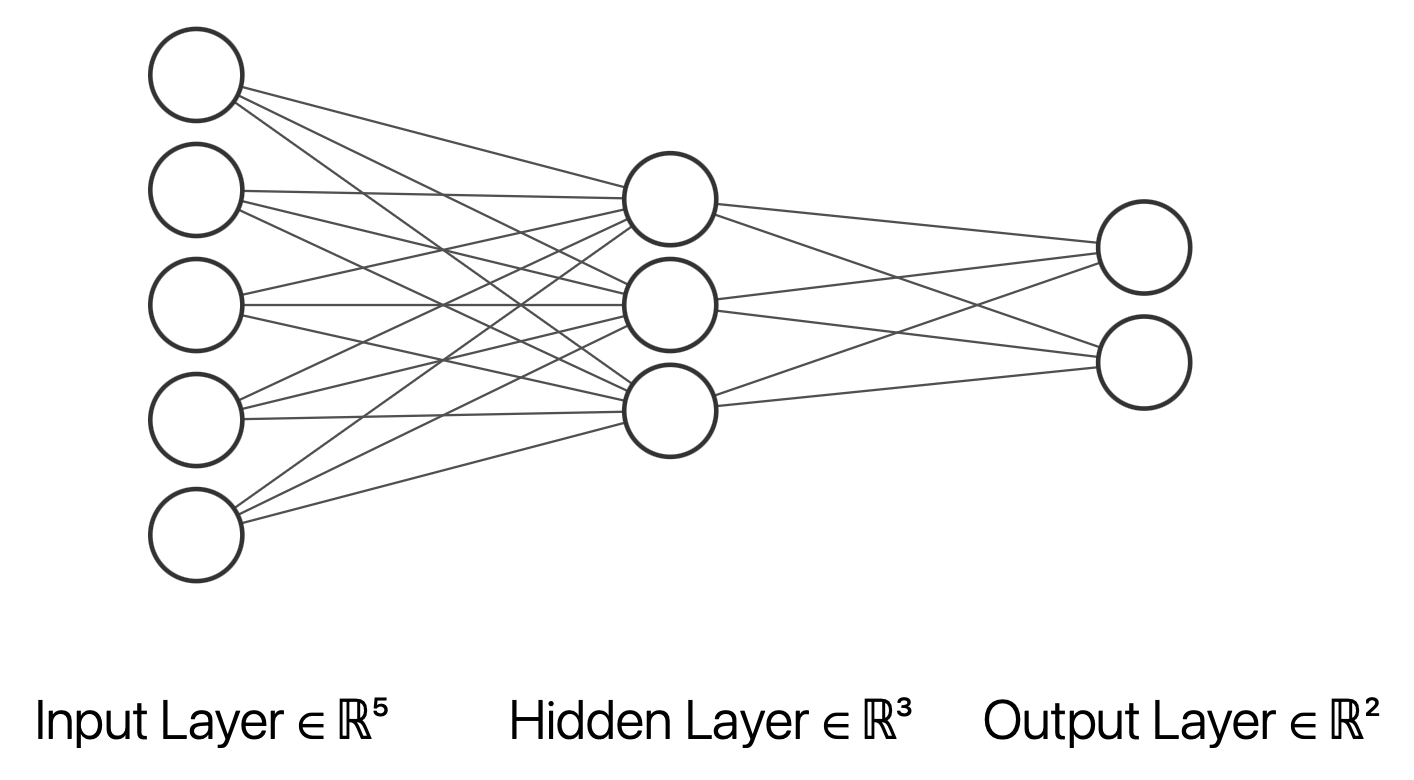
\includegraphics[scale=0.26]{FNN Visualized}}
\caption{The figure shows a simple FNN model.}
\label{fig}
\end{figure}

As shown in Figure 2, the Autoencoder (AE)\cite{Bank} model compresses (encrypts) data by bottlenecking its layers in the middle of the model and then decompressing the data (decrypts) by having mirrored layers (in size) on the other side of the bottleneck. An AE model is similar to a FNN model, except that the AE is considered a compression algorithm, as the bottleneck is able to compress inputs into just a few neurons.


\begin{figure}[htbp]
\centerline{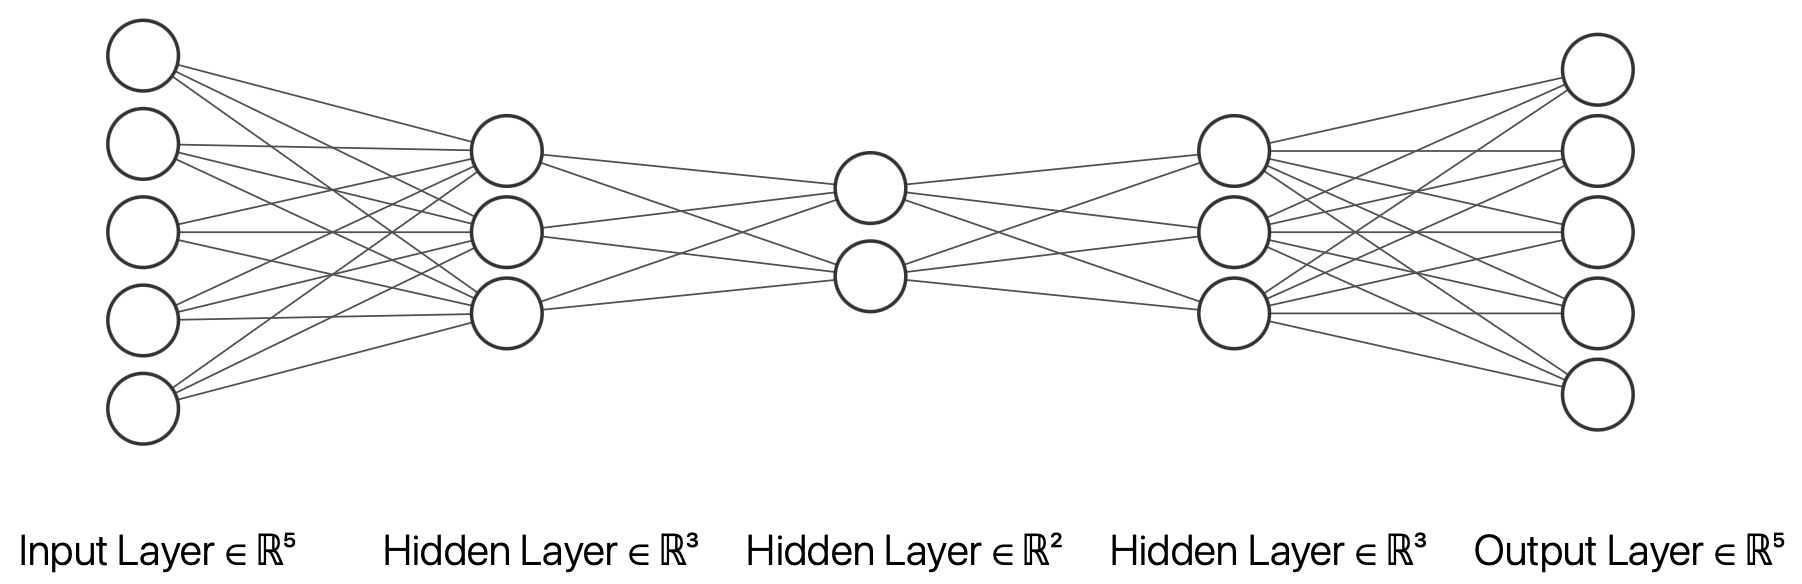
\includegraphics[scale=0.28]{AE Visualized}}
\caption{This figure depicts a simple AE, modeled after the FNN in Fig. 1. The bottleneck in the second hidden layer shows a compression from five nodes to just two.}
\label{fig}
\end{figure}

\newpage
A Convolutional Neural Network (CNN)\cite{Fukushima} model (Fig. 3)is able to compress data via kernel filters\cite{Sheikholeslami}\cite{Connault}, which is also sometimes referred to as noise reduction\cite{Garnett}. This allows the algorithm to ‘disregard’ un-important features\cite{Tomasi}, similarly to how the human brain sees things: Only what's important\cite{Hoffman}. CNN models are very popular for image classification tasks \cite{Sultana}, a famous example of a that is the LeNet-5 architecture \cite{LeCun:1}, which is able to achieve an accuracy of 99.05\% on the MNIST dataset \cite{LeCun:2}. A standard CNN model, however, just has CNN layers and is usually followed by a FNN model, which flattens and bottlenecks the output of the CNN layers, in order to be able to classify data.


\begin{figure}[htbp]
\centerline{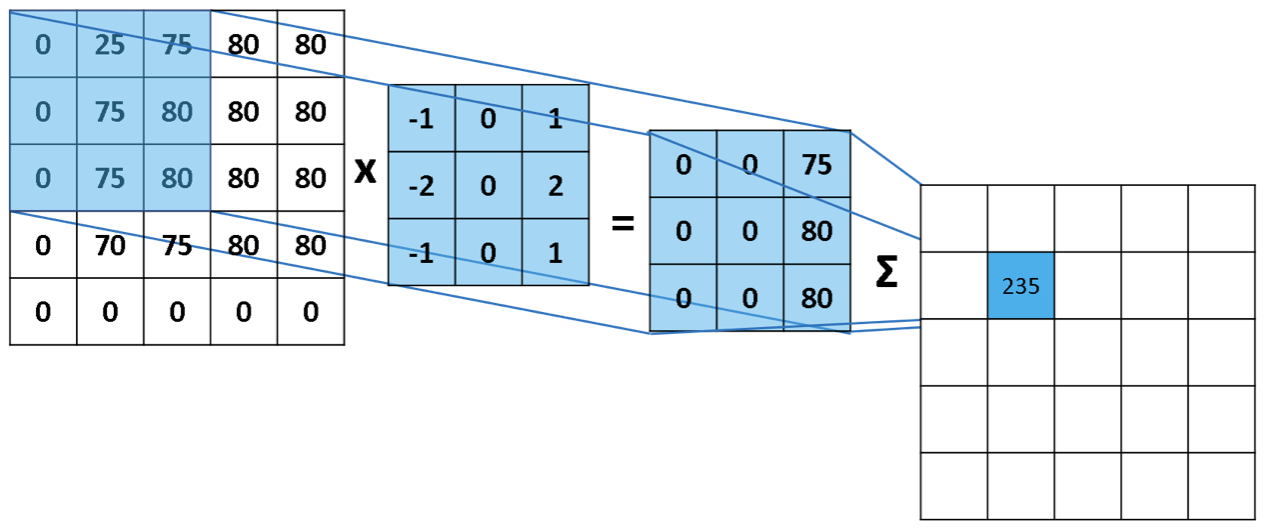
\includegraphics[scale=0.38]{CNN Visualized}}
\caption{The figure shows how a kernel filter is able to compress an image into a smaller “image.”The x and y dimension were both reduced by 2 pixels.}
\label{fig}
\end{figure}

A Long Short Term Memory Neural Network (LSTM)\cite{Hochreiter} model (Fig. 4) takes in the features of a datapoint in a sequential manner (unidirectional, dissimilar to bidirectional \cite{Cui}) and carries each feature input into its future calculations. That means, the last cell will have the “compressed” data of all previous cells to calculate a new output. This is especially useful for time-series-forecasting\cite{Elsworth} and natural language processing (NLP)\cite{Schank}, as it intelligently decides which features can be forgotten and which should be passed on as its ‘long-term’ memory\cite{Sherstinsky}.


\begin{figure}[htbp]
\centerline{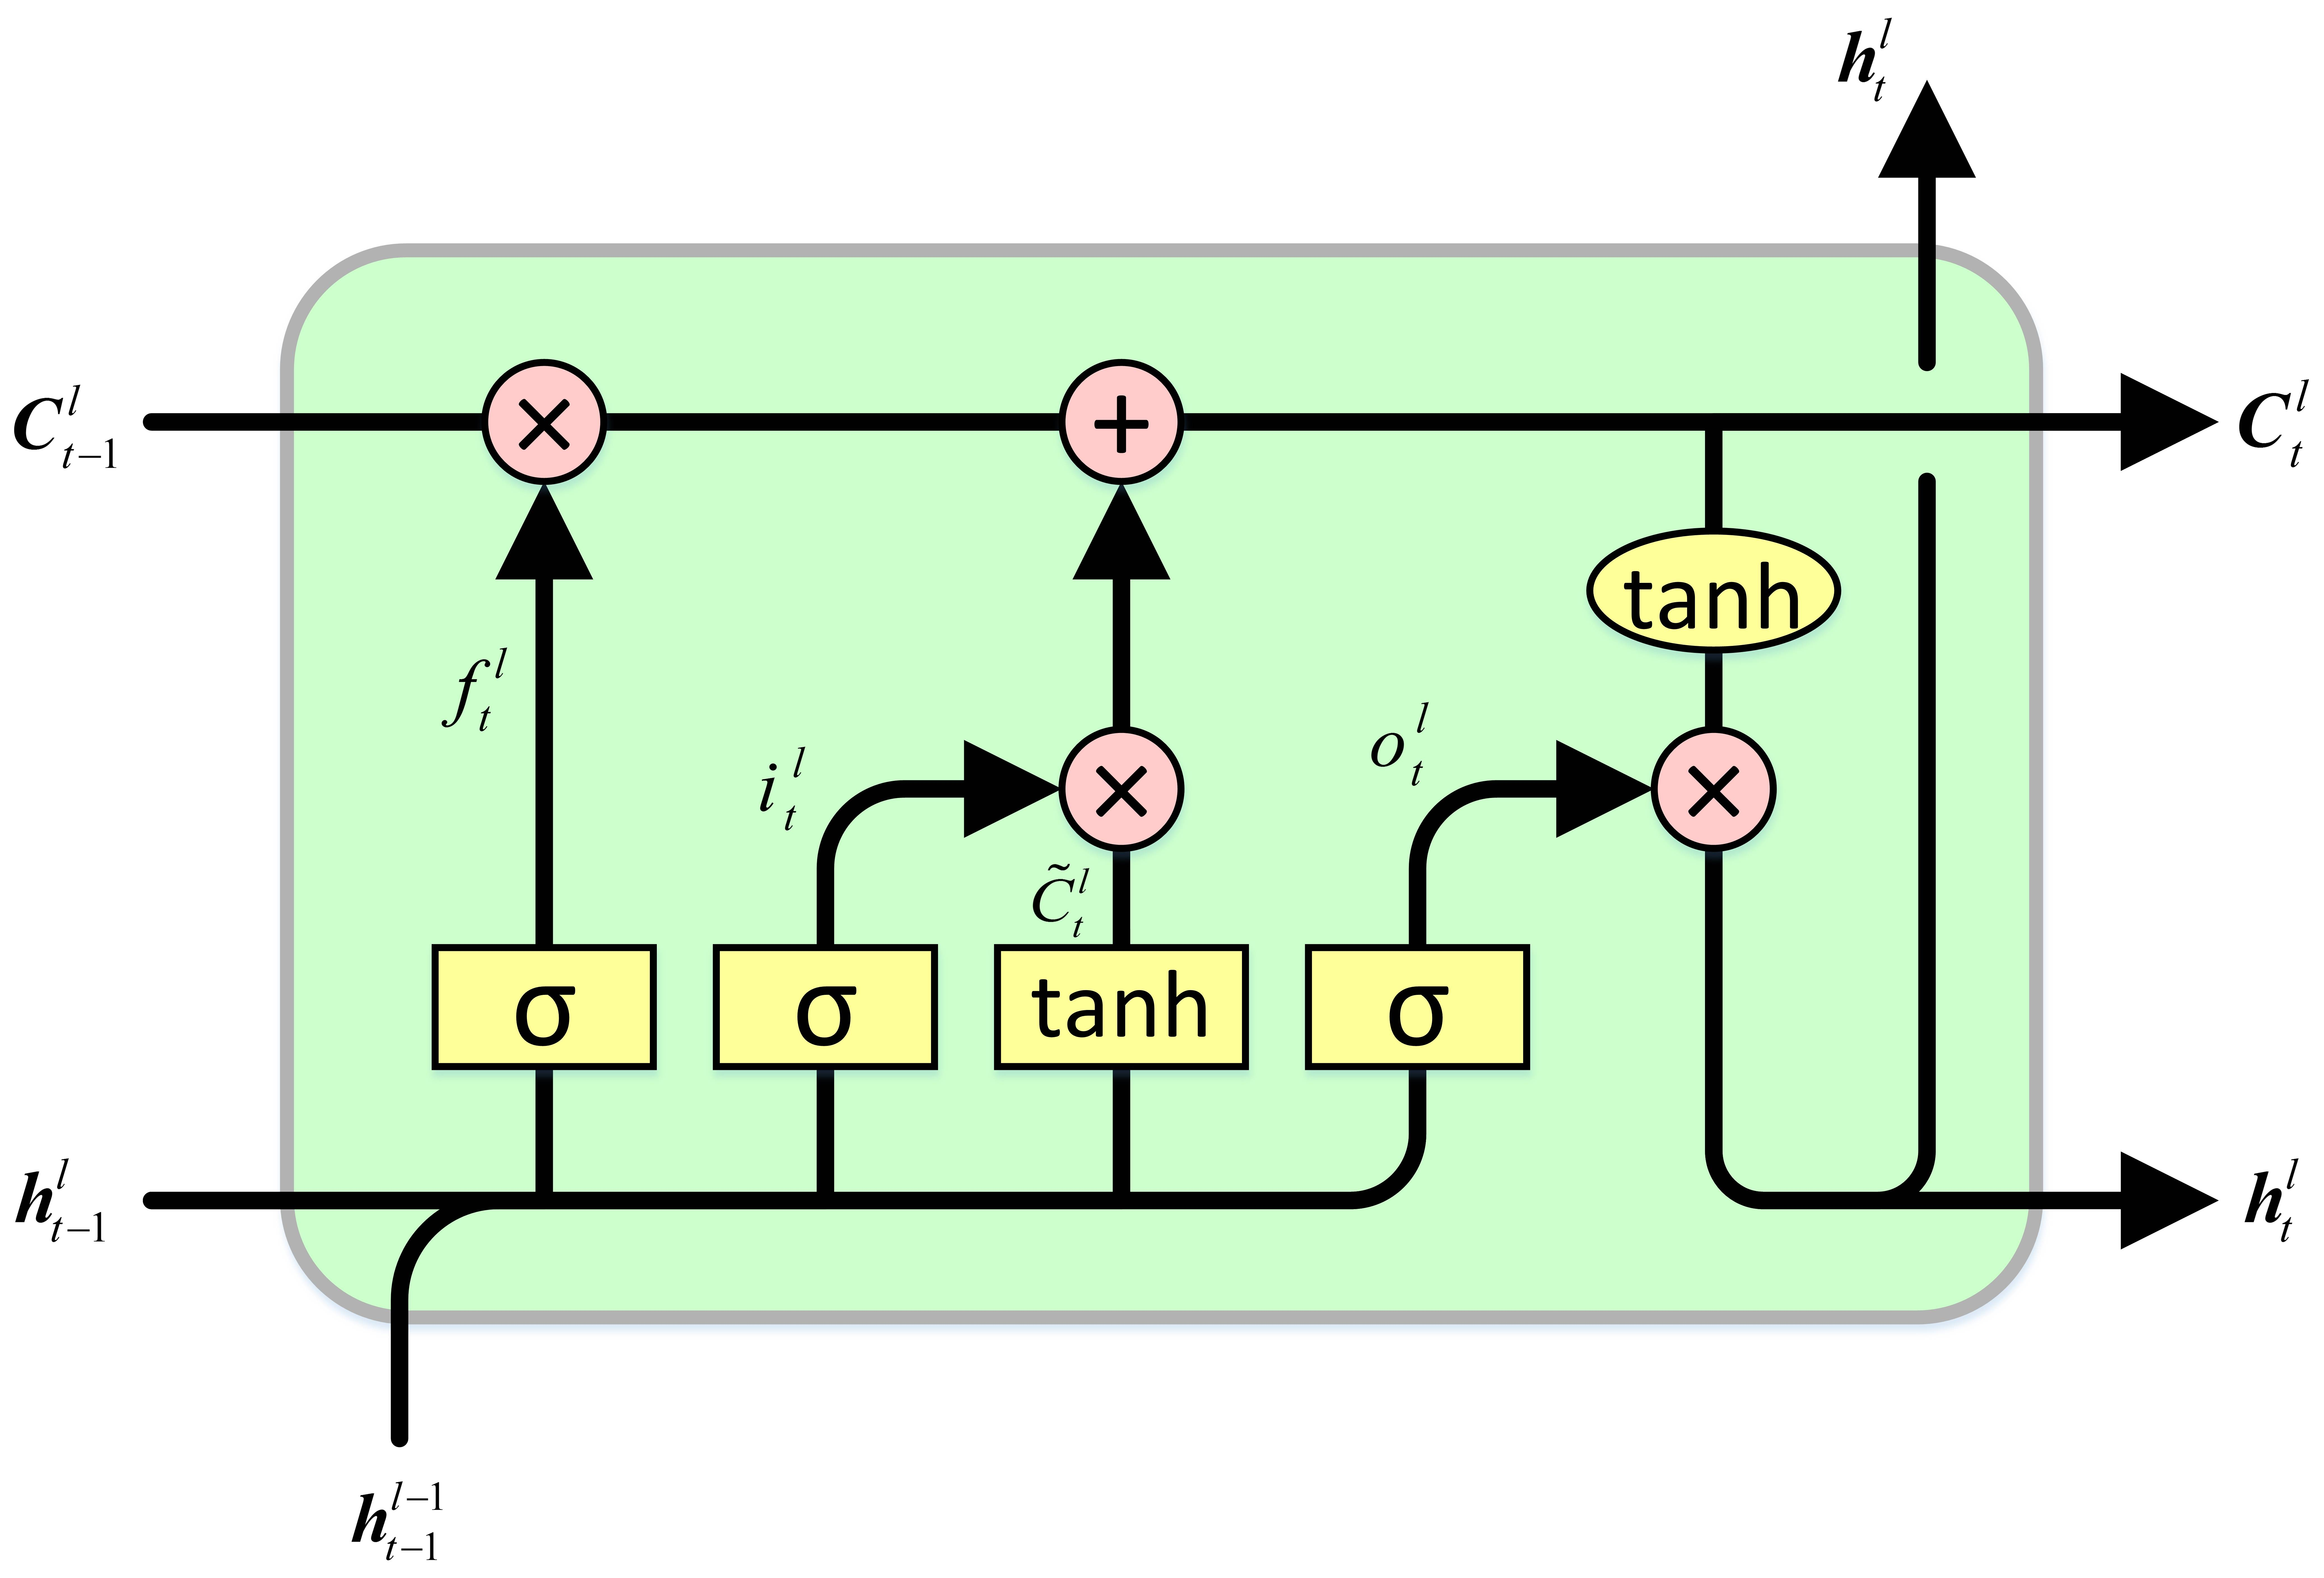
\includegraphics[scale=0.0185]{LSTM}}
\caption{A single LSTM cell, where $\sigma$ is a small FNN with the sigmoid activation function\cite{Nwankpa}, and $tanh$ is the hyperbolic tangent activation function\cite{Nwankpa}, which is also an FNN 
with $tanh$ as its activation function. The $\times$ stands for element-wise multiplication and the $+$ stands for element-wise addition. $C_t$ is the cell state, $h_t$ is the output and $l$ is for the current layer.}
\label{fig}
\end{figure}

\newpage

A Gated Recurrent Unit Neural Network (GRU)\cite{Cho} model (Fig. 5) is similar to a LSTM model, where it also tries to find connections between the features of a datapoint. It takes in the features in a sequential manner and then passes on what it thinks is useful information and disregards information through forget-gates. One big difference between LSTM cells and GRU cells, is that the GRU cells do not possess a pass-gate, which passes on the output back to the input of the next cell.

\begin{figure}[htbp]
\centerline{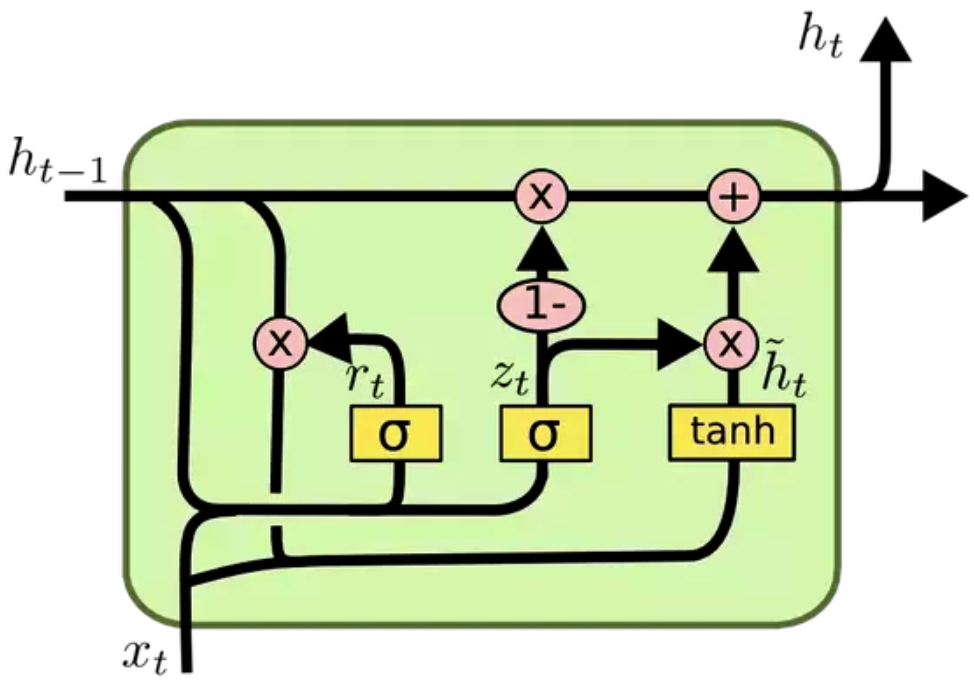
\includegraphics[scale=0.285]{GRU}}
\caption{A single GRU cell, where $\sigma$ is a small FNN with the sigmoid activation function\cite{Nwankpa}, and $tanh$ is the hyperbolic tangent activation function\cite{Nwankpa}, which is also an FNN 
with $tanh$ as its activation function. The $\times$ stands for element-wise multiplication and the $+$ stands for element-wise addition. The GRU cell is similar to the LSTM cell, but the GRU cell has two gates which are the reset and update gate.}
\label{fig}
\end{figure}


\section{Proposed Approach}
The goal of our proposed approach is to predict an organism’s kingdom and DNA type solely from its codon usage. Since the original paper was able to accomplish a high accuracy with different machine learning algorithms, which were mentioned earlier in this paper. Here we will show how different deep learning models are able to perform with the same unaltered dataset. The deep learning models we will use in this paper include the FNN, CNN, LSTM, GRU and AE. We created separate models for the kingdom classification and DNA type classification. Unlike the original paper, we used all DNA types and all kingdom classes for our classification. This means we didn’t re-classify categories that have less than 100 entries. Therefore, our datasets are comprised of eleven categories for the kingdom classification and eleven for the DNA type classification. 

The actual pre-processing of the data for each neural network architecture was quite simple. For the FNN and AE models, we were able to leave the data 'as is,' because both models require just a one dimensional stream of data as their input. 

The same goes for the inputs for the LSTM and GRU models, as they both require an one dimensional stream of data also. However, the sequence of inputs is of concern, since the closer a feature is to the output the more of an affect the feature will have on the output\cite{Rabie}. In our case, we were not able to achieve the optimal feature sequence for the LSTM and GRU models, as the possible combinations of datapoint features is $4^3!$ (or 64!)\cite{Bayer}, which is a number with 90 digits. The number of atoms in our universe is $N = 5.3 \times 10^{79}$\cite{Planck Collaboration}, which means there are far more possible combinations of feature sequences than atoms in the universe ($1.289 \times 10^{89} > 5.3 \times 10^{79}$). If we tried to find the optimal connection between features for the LSTM and GRU network, the sun would explode before we finished\cite{Krauss}. Therefore, instead of actively looking for the best feature shuffle, we simply stuck with the already given sequence of features.

However, for the CNN model in this paper, we had to reshape the feature sequence from one dimensional to two dimensional\cite{Ghosh}. This is because the architecture we used for the CNN model required us to feed it two dimensional input data, or image data. This meant we had to reshape the input data to be an $8 \times 8$ image. The image itself just looks like some black and white dots, as shown in Fig. 6. 

\begin{figure}[htbp]
\centerline{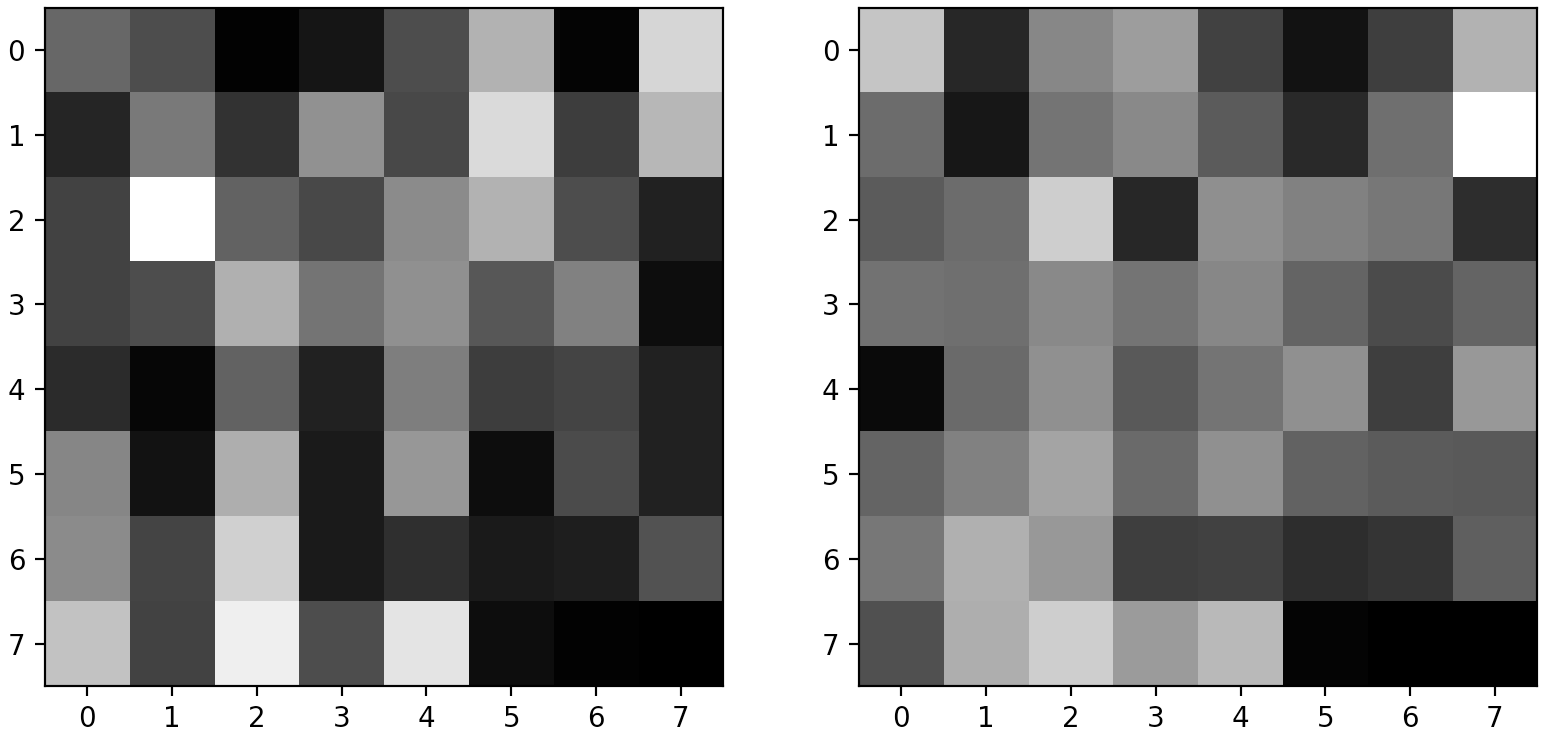
\includegraphics[scale=0.26]{Codon Display}}
\caption{Shows the $1^{st}$ and $100^{th}$ genome of the Codon Usage dataset as an $8 \times 8$ image.}
\label{fig}
\end{figure}

As for the model evaluation, we also chose a 80/20 split for the training and testing data respectively. We built five models for both classification tasks, and evaluated them on the three datasets. This means, we evaluated a total of 30 models. To find the best hyper-parameters for the FNN, CNN, LSTM, GRU and AE models, we had to try different architectures to create the highest accuracy for each model. 
For creating the different architectures we used the open source framework: TensorFlow. TensorFlow allowed us to build complex deep learning models within minutes and to start the training process right away. Additionally, us using TensorFlow will facilitate reproducibility, as TensorFlow is a standardized framework that can run on almost any machine. All of the code is made public on Lennart Buhl’s GitHub account: \url{https://github.com/Lennart2001/codon-usage/blob/main/Python\%20Code/codon\_usage.py}.


\section{Results}
The results of our training for the FNN, CNN, LSTM, GRU and AE models are displayed below. Unlike the original paper, we are showing six different tables, which correspond to the three datasets times the two classification tasks. The best value for kingdom classification from table \rom{1},\rom{2} and \rom{3} is achieved by dropped rows with accuracy of 95.7\% by FNN. Similarly the best value for DNA type classification from table \rom{4}, \rom{5} and \rom{6} is achieved by dropped rows with accuracy of 99.51\% by FNN. 


\begin{table}[htbp]

\begin{center}
\caption{Kingdom Classification - Dropped}

\begin{tabular}{|c|c|c|c|}
\hline
& Macro F1-Score& Micro F1-Score& Accuracy \\
\hline
FNN& 0.8935& 0.9570& \textbf{0.9570}\\

CNN& 0.8157& 0.9340& 0.9341\\

LSTM& 0.3250& 0.4589& 0.4589\\

GRU& 0.7321& 0.8956& 0.8956\\

AE& 0.6161& 0.8987& 0.8987\\
\hline
\end{tabular}
\end{center}

\begin{center}
\caption{Kingdom Classification - Mean}
\begin{tabular}{|c|c|c|c|}
\hline
& Macro F1-Score& Micro F1-Score& Accuracy \\
\hline
FNN& 0.7868& 0.9325& \textbf{0.9329}\\

CNN& 0.7730& 0.9267& 0.9267\\

LSTM& 0.5738& 0.7467& 0.7467\\

GRU& 0.7189& 0.8910& 0.8910\\

AE& 0.5356& 0.8956& 0.8956\\
\hline
\end{tabular}
\end{center}


\begin{center}
\caption{Kingdom Classification - Median}
\begin{tabular}{|c|c|c|c|}
\hline
& Macro F1-Score& Micro F1-Score& Accuracy \\
\hline
FNN& 0.8044& 0.9413& \textbf{0.9413}\\

CNN& 0.7688& 0.9156& 0.9156\\

LSTM& 0.3449& 0.5553& 0.5553\\

GRU& 0.6965& 0.8872& 0.8872\\

AE& 0.5429& 0.8956& 0.8956\\
\hline
\end{tabular}
\end{center}

\begin{center}
\caption{DNA Type Classification - Dropped}
\begin{tabular}{|c|c|c|c|}
\hline
& Macro F1-Score& Micro F1-Score& Accuracy \\
\hline
FNN& 0.3279& 0.9927& 0.9927\\

CNN& 0.4412& 0.9951& \textbf{0.9951}\\

LSTM& 0.3272& 0.9919& 0.9919\\

GRU& 0.3259& 0.9908& 0.9908\\

AE& 0.3279& 0.9931& 0.9931\\
\hline
\end{tabular}
\end{center}


\begin{center}
\caption{DNA Type Classification - Mean}
\begin{tabular}{|c|c|c|c|}
\hline
& Macro F1-Score& Micro F1-Score& Accuracy \\
\hline
FNN& 0.5464& 0.9942& \textbf{0.9942}\\

CNN& 0.4920& 0.9889& 0.9885\\

LSTM& 0.4138& 0.9858& 0.9858\\

GRU& 0.5054& 0.9942& \textbf{0.9942}\\

AE& 0.4929& 0.9931& 0.9931\\
\hline
\end{tabular}
\end{center}

\begin{center}
\caption{DNA Type Classification - Median}
\begin{tabular}{|c|c|c|c|}
\hline
& Macro F1-Score& Micro F1-Score& Accuracy \\
\hline
FNN& 0.5574& 0.9939& \textbf{0.9939}\\

CNN& 0.4630& 0.9923& 0.9919\\

LSTM& 0.5612& 0.9923& 0.9923\\

GRU& 0.4927& 0.9931& 0.9931\\

AE& 0.4927& 0.9939& \textbf{0.9939}\\
\hline
\end{tabular}
\end{center}

\end{table}

\newpage

Comparing the five different kinds of neural networks against each other, the non-time-series neural networks appear to be more accurate when classifying the kingdom datasets, as shown in table \rom{1}, table \rom{2} and table \rom{3}. This is because they either compress the data or just learn the datapoints as a whole, rather than try to find connections between the codons and draw conclusions from the correlations between them\cite{Elsworth}. However, for the DNA type classification, all neural networks appeared to be similar in accuracy (tables \rom{4}-\rom{6}), with the slight performance lead going to the non-time-series neural networks. 

Therefore, it is clear that the best performance overall came from the FNN, AE and the CNN neural network models. The LSTM and GRU models performed the worst(as seen in table \rom{1},\rom{2} \& \rom{3}), which is expected as they learn from the correlations between codons, rather than the codons as a whole. The GRU model performed slightly better as the LSTM model(tables \rom{1} - \rom{3}, \rom{5} \& \rom{6}), because GRU models are able to converge faster as they have a less complex structure, thereby being computationally more efficient\cite{Chung}. 


\section{Conclusions}
When comparing the outcome of the three datasets, it is worth noting how the two datapoints, which had missing values, had an effect on the models’ learning process. The dropping of the datapoints produced an increase in accuracy of approximately 1.3\% and 2\% for the CNN and FNN, respectively, for the kingdom classification (table \rom{1} vs table \rom{2} \& \rom{3}). Without dropping these datapoints, the models had a slightly higher difficulty at learning the dataset. However, the average overall performance of all models was slightly better without dropping any values for the DNA type classification. Yet, the best results were still produced by the FNN, CNN and AE algorithm, which is verifiable by the tables \rom{1}-\rom{6}. 

We were able to reproduce the findings of the original paper and were able to produce an even higher accuracy for the kingdom classification with an accuracy of 95.7\% (table \rom{1}) achieved by the FNN algorithm compared to the 91.32\% of the original paper’s FNN. We were also able to produce a higher accuracy for the DNA type classification using the CNN model, which produced an accuracy of 99.51\% (table \rom{4}) compared to the 99.15\% accuracy of the original paper’s FNN. Furthermore, the CNN model did not only beat the original paper’s FNN accuracy record of 99.15\%, but it also achieved an accuracy that was unmatched by any other algorithm suggested by the original paper. Therefore, it is clear that by using a dataset without reclassification and with dropping the rows with missing values, one will be able to produce models that have a much higher accuracy, than with the biased dataset of the original paper. 

%% NEWLY ADDED %% 

The ability to predict an organism's TI and GC, based on their codon usage bias levels, is very important in the domain of healthcare and biomedicine. Imagine we detect a new organism, that doesn't look like anything we have ever seen before. As demonstrated in this paper, it is very possible to predict the TI and GC of an organism (even if it has never been seen before), or rather, which TI and GC the organism is most closely related to. This will not only speed up the classification of new organisms, but it also opens the door for other classification models, where researchers are able to identify common ancestors of different organisms, based on their codon usages. Or simply find relations between, previously believed to be unrelated, organisms.

Additionally, through the extensive outlining of codon bias usage levels in humans, it will be possible to predict whether a person has any genetic predispositions regarding diseases or substances. Deep learning models will play a vital role in these predictions, as they will make it easy for doctors to interpret the results of a patient's gene expressions. Researchers and doctors will be able to utilize artificial intelligence to treat people with more effective medications, tailored to the patient's (potentially yet undiagnosed) genetic predispositions. Unlocking the hidden information gold-mine that lays within us, has the potential to help all of humanity, by revolutionizing how we prescribe medical treatments and give diagnoses to people.  


%% NEWLY ADDED %% 


\section*{Acknowledgment}
I would like to thank Dr. Sayantica Pattanayak for encouraging me to do research in the field of artificial intelligence, as well as encouraging me to write my findings up into a paper. Going into studying artificial Intelligence can be scary at first, but with the help of Dr. Pattanayak I was able to not only learn, but even develop a fondness for the complexity that A.I. is. 

\begin{thebibliography}{00}

\bibitem{Khomtchouk} B. B. Khomtchouk, “Codon usage bias levels predict taxonomic identity and genetic composition,” bioRxiv, 01-Jan-2020. \url{https://doi.org/10.1101/2020.10.26.356295}. 
\bibitem{Tedersoo} L. Tedersoo, “Proposal for practical multi-kingdom classification of eukaryotes based on monophyly and comparable divergence time criteria,” bioRxiv, 01-Jan-2017. \url{https://www.biorxiv.org/content/10.1101/240929v1.full}.
\bibitem{Codon Dataset} B. B. Khomtchouk, “Codon Usage Data Set ,” UCI Machine Learning Repository: Codon Usage Data Set. \url{https://archive.ics.uci.edu/ml/datasets/Codon+usage}. 
\bibitem{Ray} T. Ray, “Google says 'exponential' growth of AI is changing nature of compute,” ZDNET, 01-Nov-2018. \url{https://www.zdnet.com/article/google-says-exponential-growth-of-ai-is-changing-nature-of-compute/}. 
\bibitem{Kumar} Y. Kumar, A. Koul, R. Singla, and M. F. Ijaz, “Artificial Intelligence in disease diagnosis: A systematic literature review, synthesizing framework and future research agenda,” Journal of ambient intelligence and humanized computing, 13-Jan-2022. \url{https://www.ncbi.nlm.nih.gov/pmc/articles/PMC8754556/}. 
\bibitem{Deng} J. Deng, Z. Yang, I. Ojima, D. Samaras, and F. Wang, “Artificial Intelligence in drug discovery: Applications and techniques,” arXiv.org, 02-Nov-2021. \url{https://arxiv.org/abs/2106.05386}. 
\bibitem{Paul} D. Paul, G. Sanap, S. Shenoy, D. Kalyane, K. Kalia, and R. K. Tekade, “Artificial Intelligence in drug discovery and development,” Drug discovery today, Jan-2021. \url{https://www.ncbi.nlm.nih.gov/pmc/articles/PMC7577280/}. 
\bibitem{Li} J. Li, “Recent advances in end-to-end automatic speech recognition,” arXiv.org, 02-Feb-2022. \url{https://arxiv.org/abs/2111.01690}. 
\bibitem{Briganti} G. Briganti and O. Le Moine, “Artificial Intelligence in medicine: Today and Tomorrow,” Frontiers, 05-Feb-2020. \url{https://www.frontiersin.org/articles/10.3389/fmed.2020.00027/full}. 
\bibitem{Davenport} T. Davenport and R. Kalakota, “The potential for artificial intelligence in Healthcare,” Future healthcare journal, Jun-2019. \url{https://www.ncbi.nlm.nih.gov/pmc/articles/PMC6616181/}. 
\bibitem{Rahmani} A. M. Rahmani, E. Azhir, S. Ali, M. Mohammadi, O. H. Ahmed, M. Yassin Ghafour, S. Hasan Ahmed, and M. Hosseinzadeh, “Artificial Intelligence Approaches and mechanisms for Big Data Analytics: A systematic study,” PeerJ. Computer science, 14-Apr-2021. \url{https://www.ncbi.nlm.nih.gov/pmc/articles/PMC8053021/}. 
\bibitem{Rajpurkar} P. Rajpurkar, J. Irvin, K. Zhu, B. Yang, H. Mehta, T. Duan, D. Ding, A. Bagul, C. Langlotz, K. Shpanskaya, M. P. Lungren, and A. Y. Ng, “CheXNet: Radiologist-level pneumonia detection on chest X-rays with deep learning,” arXiv.org, 25-Dec-2017. \url{https://arxiv.org/abs/1711.05225}. 
\bibitem{Parvathy} S. T. Parvathy, V. Udayasuriyan, and V. Bhadana, “Codon usage bias,” Molecular biology reports, 25-Nov-2021. \url{https://www.ncbi.nlm.nih.gov/pmc/articles/PMC8613526/}. 
\bibitem{Kooning} E. V. Kooning and A. S. Novozhilov, “Origin and evolution of the Genetic Code: The universal enigma,” IUBMB life. \url{https://pubmed.ncbi.nlm.nih.gov/19117371/}. 
\bibitem{Zhou} Z. Zhou, Y. Dang, and M. Zhou, “Codon usage is an important determinant of gene expression levels largely through its effects on transcription.” \url{https://www.pnas.org/doi/10.1073/pnas.1606724113}. 
\bibitem{Fu} H. Fu , Y. Liang, X. Zhong, Z. Pan, L. Huang, H. Zhang, Y. Xu, W. Zhou, and Z. Liu, “Codon optimization with deep learning to enhance protein expression,” Scientific reports, 19-Oct-2020. \url{https://pubmed.ncbi.nlm.nih.gov/33077783/}. 
\bibitem{Hochreiter} S. Hochreiter and J. Schmidhuber, “Long Short-Term Memory.” \url{http://www.bioinf.jku.at/publications/older/2604.pdf}.
\bibitem{Cui} Z. Cui, R. Ke, Z. Pu, and Y. Wang, “Deep bidirectional and unidirectional LSTM recurrent neural network for network-wide traffic speed prediction,” arXiv.org, 23-Nov-2019. \url{https://arxiv.org/abs/1801.02143}.
\bibitem{Mehrabi} N. Mehrabi, F. Morstatter, N. Saxena, K. Lerman, and A. Galstyan, “A survey on bias and fairness in machine learning.” \url{https://arxiv.org/pdf/1908.09635v2.pdf}. 
\bibitem{Krenker} A. Krenker, J. Bešter, and A. Kos, “Introduction to the Artificial Neural Networks,” IntechOpen, 11-Apr-2011. \url{https://www.intechopen.com/chapters/14881}. 
\bibitem{Cunningham} P. Cunningham and S. J. Delany, “K-nearest neighbour classifiers: 2nd edition (with python examples),” arXiv.org, 29-Apr-2020. \url{https://arxiv.org/abs/2004.04523}. 
\bibitem{Breiman} L. Breiman, “Random forests - Machine Learning,” SpringerLink, 2001. \url{https://link.springer.com/article/10.1023/A:1010933404324}. 
\bibitem{Chen} T. Chen and C. Guestrin, “XGBoost: A scalable tree boosting system,” arXiv.org, 10-Jun-2016. \url{https://arxiv.org/abs/1603.02754}. 
\bibitem{Mitchell} T. M. Mitchell, Machine Learning. 1997. pp. 177–198. McGraw Hill, New York, NY
\bibitem{Zhu} J. Zhu, “Probabilistic Machine Learning: Models, algorithms and a programming library,” Probabilistic Machine Learning: Models, Algorithms and a Programming Library | IJCAI, 01-Jan-1970. \url{https://doi.org/10.24963/ijcai.2018/823}. 
\bibitem{Grinberg} N. F. Grinberg, O. I. Orhobor, and R. D. King, “An evaluation of machine-learning for predicting phenotype: studies in yeast, rice, and wheat,” SpringerLink, 23-Oct-2019. \url{https://link.springer.com/article/10.1007/s10994-019-05848-5}. 
\bibitem{Tian} J. Tian, Y. Yan, Q. Yue, X. Liu, X. Chu, N. Wu, and Y. Fan, “Predicting synonymous codon usage and optimizing the heterologous gene for expression in E. coli,” Nature News, 30-Aug-2017. \url{https://www.nature.com/articles/s41598-017-10546-0}. 
\bibitem{Hurley} J. M. Hurley and J. C. Dunlap, “A fable of too much too fast,” Nature News, 17-Feb-2013. \url{https://www.nature.com/articles/nature11952}. 
\bibitem{GenBank} “GenBank,” National Center for Biotechnology Information. \url{https://www.ncbi.nlm.nih.gov/genbank/}. 
\bibitem{Lee} J.-Y. Lee, N. C. Sadler, R. G. Egbert, C. R. Anderton, K. S. Hofmockel, J. K. Jansson, and H.-S. Song, “Deep Learning predicts microbial interactions from self-organized spatiotemporal patterns,” Computational and Structural Biotechnology Journal, 29-May-2020. \url{https://www.sciencedirect.com/science/article/pii/S2001037020302865}. 
\bibitem{Kroll} A. Kroll, M. K. M. Engqvist, D. Heckmann, and M. J. Lercher, “Deep learning allows genome-scale prediction of Michaelis constants from structural features,” PLOS Biology. \url{https://journals.plos.org/plosbiology/article?id=10.1371\%2Fjournal.pbio.3001402}. 
\bibitem{Washburn} J. D. Washburn, M. K. Mejia-Guerra, G. Ramstein, K. A. Kremling, R. Valluru, E. S. Buckler, and H. Wang, “Evolutionarily informed deep learning methods for predicting relative transcript abundance from DNA sequence,” Proceedings of the National Academy of Sciences of the United States of America. \url{https://pubmed.ncbi.nlm.nih.gov/30842277/}. 
\bibitem{Dastres} R. Dastres and M. Soori, “Artificial Neural Network Systems.” \url{https://hal.archives-ouvertes.fr/hal-03349542/document}. 
\bibitem{Taskar} B. Taskar, E. Segal, and D. Koller, “Probabilistic classification and clustering in relational data.” \url{https://ai.stanford.edu/users/koller/Papers/Taskar+al:IJCAI01.pdf} 
\bibitem{Sarker} I. H. Sarker, “Machine Learning: Algorithms, Real-World Applications and Research Directions,” SpringerLink, 22-Mar-2021. \url{https://link.springer.com/article/10.1007/s42979-021-00592-x}. 
\bibitem{Sirignano} J. Sirignano and K. Spiliopoulos, “DGM: A deep learning algorithm for solving partial differential equations,” arXiv.org, 05-Sep-2018. \url{https://arxiv.org/abs/1708.07469}. 
\bibitem{Maennel} H. Maennel, I. Alabdulmohsin, I. Tolstikhin, R. J. N. Baldock, O. Bousquet, S. Gelly, and D. Keysers, “What do neural networks learn when trained with random labels?,” arXiv.org, 11-Nov-2020. \url{https://arxiv.org/abs/2006.10455}. 
\bibitem{Patel} P. Patel, M. Nandu, and P. Raut, “Initialization of Weights in Neural Networks.” \url{https://www.researchgate.net/publication/330875010_Initialization_of_Weights_in_Neural_Networks}.
\bibitem{Bank} D. Bank, N. Koenigstein, and R. Giryes, “Autoencoders,” arXiv.org, 03-Apr-2021. \url{https://arxiv.org/abs/2003.05991}.
\bibitem{Fukushima} K. Fukushima, “Neocognitron: A Self-organizing Neural Network Model for a Mechanism of Pattern Recognition Unaffected by Shift in Position.,” 1980. \url{https://www.rctn.org/bruno/public/papers/Fukushima1980.pdf}. 
\bibitem{Sheikholeslami} F. Sheikholeslami, D. Berberidis, and G. B. Giannakis, “Large-scale kernel-based feature extraction via budgeted nonlinear subspace tracking,” arXiv.org, 26-Dec-2017. \url{https://arxiv.org/abs/1601.07947}. 
\bibitem{Connault} B. Connault, “Kernel Filtering.” \url{https://www.sas.upenn.edu/~connault/kernel-filtering.pdf}. 
\bibitem{Garnett} R. Garnett, T. Huegerich, C. Chui, and W. He, “A universal noise removal algorithm with an impulse detector.” \url{http://www.cs.umsl.edu/~he/papers/ieeeroad.pdf}. 
\bibitem{Tomasi} C. Tomasi and R. Manduchi, "Bilateral filtering for gray and color images," Sixth International Conference on Computer Vision (IEEE Cat. No.98CH36271), 1998, pp. 839-846, doi: 10.1109/ICCV.1998.710815. \url{https://users.soe.ucsc.edu/~manduchi/Papers/ICCV98.pdf}.
\bibitem{Hoffman} D. D. Hoffman, “Human Vision as a Reality Engine,” Human vision as a reality engine - University of California, Irvine. \url{http://www.cogsci.uci.edu/~ddhoff/HoffmanFABBS.pdf}.
\bibitem{Sultana} F. Sultana, A. Sufian, and P. Dutta, “Advancements in image classification using convolutional neural network,” arXiv.org, 08-May-2019. \url{https://arxiv.org/abs/1905.03288}. 
\bibitem{LeCun:1} Y. LeCun, “Gradient-Based Learning Applied to Document Recognition." \url{http://yann.lecun.com/exdb/publis/pdf/lecun-01a.pdf}.
\bibitem{LeCun:2} Y. LeCun, C. Cortes, and C. J. C. Burges, “MNIST” The MNIST Database of handwritten digits. \url{http://yann.lecun.com/exdb/mnist/}. 
\bibitem{Elsworth} S. Elsworth and S. Güttel, “Time Series forecasting using LSTM networks: A symbolic approach,” arXiv.org, 12-Mar-2020. \url{https://arxiv.org/abs/2003.05672}. 
\bibitem{Schank} R. C. Schank and L. Tesler, “A conceptual dependency parser for natural language,” ACL Anthology. \url{https://aclanthology.org/C69-0201.pdf}. 
\bibitem{Sherstinsky} A. Sherstinsky, “Fundamentals of Recurrent Neural Network (RNN) and long short-term memory (LSTM) network,” arXiv.org, 21-Dec-2020. \url{https://arxiv.org/abs/1808.03314v8}. 
\bibitem{Nwankpa} C. Nwankpa, W. Ijomah, A. Gachagan, and S. Marshall, “Activation functions: Comparison of trends in practice and research for Deep Learning,” arXiv.org, 08-Nov-2018. \url{https://arxiv.org/abs/1811.03378}. 
\bibitem{Cho} K. Cho, B. van Merrienboer, D. Bahdanau, and Y. Bengio, “On the properties of neural machine translation: Encoder-decoder approaches,” arXiv.org, 07-Oct-2014. \url{https://arxiv.org/abs/1409.1259}. 
\bibitem{Rabie} H. Rabie, M. El-Beltagy, A. Tharwat, and S. A. Hassan, “Exploring input selection for time series forecasting.” \url{https://www.researchgate.net/publication/220705175_Exploring_Input_Selection_for_Time_Series_Forecasting}. 
\bibitem{Bayer} D. Bayer and P. Diaconis, “Trailing The Dovetail Shuffle To Its Lair.” \url{https://statweb.stanford.edu/~cgates/PERSI/papers/bayer92.pdf}. 
\bibitem{Planck Collaboration} P. A. R. Ade, N. Aghanim, M. Arnaud, M. Ashdown, J. Aumont, “Planck 2015 results. XIII. cosmological parameters,” NASA/ADS. \url{https://doi.org/10.1051\%2F0004-6361\%2F201525830}. 
\bibitem{Krauss} L. M. Krauss and G. D. Starkman, “Life, the universe, and nothing: Life and death in an ever-expanding universe,” arXiv.org, 12-Feb-1999. \url{https://arxiv.org/abs/astro-ph/9902189}. 
\bibitem{Ghosh} S. Ghosh, N. Das, and M. Nasipuri, “Reshaping inputs for convolutional neural network: Some common and uncommon methods.” \url{https://doi.org/10.1016/j.patcog.2019.04.009}. 
\bibitem{Chung} J. Chung, C. Gulcehre, K. H. Cho, and Y. Bengio, “Empirical evaluation of gated recurrent neural networks on sequence modeling,” arXiv.org, 11-Dec-2014. \url{https://arxiv.org/abs/1412.3555v1}. 

\end{thebibliography}
\vspace{12pt}


\end{document}
